
% This LaTeX was auto-generated from MATLAB code.
% To make changes, update the MATLAB code and republish this document.

\documentclass{article}
\usepackage{graphicx}
\usepackage{color}

\sloppy
\definecolor{lightgray}{gray}{0.5}
\setlength{\parindent}{0pt}

\begin{document}

    
    
\subsection*{Contents}

\begin{itemize}
\setlength{\itemsep}{-1ex}
   \item Questiomn 1: Howard Policy Improvement and Endogenous Grid Method
   \item Quesion 1: Endogenous Grid Method
   \item Question 2: Stationary Distribution and Income Fluctuations
\end{itemize}
\begin{verbatim}
% Econ 527 Spring 2026
% HW 3
% Professor Greaney
% Written by: Camille Bergeron
% Due: May 08, 2026
% Last Edited: May 06, 2026
\end{verbatim}


\subsection*{Questiomn 1: Howard Policy Improvement and Endogenous Grid Method}

\begin{verbatim}
run('programs/PS3_Q1_HPI.m'); % run Howard policy improvement code
\end{verbatim}

        \color{lightgray} \begin{verbatim}Wealth grid points:
  Columns 1 through 7

         0    0.0051    0.0204    0.0459    0.0816    0.1275    0.1837

  Columns 8 through 10

    0.2500    0.3265    0.4132

Transition probabilities:
    0.8145    0.1715    0.0135    0.0005    0.0000
    0.0429    0.8213    0.1290    0.0068    0.0001
    0.0023    0.0860    0.8235    0.0860    0.0023
    0.0001    0.0068    0.1290    0.8213    0.0429
    0.0000    0.0005    0.0135    0.1715    0.8145

Running Howard policy improvement with max policy iterations = 5...
File does not exist. Running Howard policy improvement...
Convergence achieved after 34 iterations with convergence error: 3.7744e-06
Completed Howard policy improvement with max policy iterations = 5 in 9.4046 seconds
Running Howard policy improvement with max policy iterations = 10...
File does not exist. Running Howard policy improvement...
Convergence achieved after 23 iterations with convergence error: 3.082e-06
Completed Howard policy improvement with max policy iterations = 10 in 7.9696 seconds
Running Howard policy improvement with max policy iterations = 20...
File does not exist. Running Howard policy improvement...
Convergence achieved after 15 iterations with convergence error: 2.1535e-06
Completed Howard policy improvement with max policy iterations = 20 in 7.1523 seconds
    5.0000    9.4046   34.0000
   10.0000    7.9696   23.0000
   20.0000    7.1523   15.0000

\end{verbatim} \color{black}
    

\subsection*{Quesion 1: Endogenous Grid Method}

\begin{verbatim}
run('programs/PS3_Q1_EGM.m'); % run Endogenous Grid Method code
\end{verbatim}

        \color{lightgray} \begin{verbatim}Iteration  100,  error = 1.3113e+25
Iteration  200,  error = 1.4232e+49
Iteration  300,  error = 9.0403e+71
Iteration  400,  error = 3.1889e+95
Iteration  500,  error = 1.1756e+119
Iteration  600,  error = 4.3718e+142
Iteration  700,  error = 1.5134e+166
Iteration  800,  error = 9.5523e+189
Iteration  900,  error = 4.3852e+215
Iteration 1000,  error = 8.0964e+236
Iteration 1100,  error = 1.8564e+260
Iteration 1200,  error = 1.1019e+284
Iteration 1300,  error = 3.7035e+304
Iteration 1400,  error = 7.0795e+304
Iteration 1500,  error = 1.8767e+303
Iteration 1600,  error = 9.0877e+299
Iteration 1700,  error = 1.5141e+305
Iteration 1800,  error = 1.8966e+298
Iteration 1900,  error = 1.9558e+301
Iteration 2000,  error = 8.3415e+303
Iteration 2100,  error = 1.3446e+297
Iteration 2200,  error = 5.1220e+299
Iteration 2300,  error = 1.9481e+302
Iteration 2400,  error = 7.4075e+304
EGM converged after 2433 iterations in 1.43 seconds (error = 0.00e+00)
\end{verbatim} \color{black}
    

\subsection*{Question 2: Stationary Distribution and Income Fluctuations}

\begin{verbatim}
run('programs/PS3_Q2.m')
\end{verbatim}

        \color{lightgray} \begin{verbatim}Transition probabilities:
    0.8145    0.1715    0.0135    0.0005    0.0000
    0.0429    0.8213    0.1290    0.0068    0.0001
    0.0023    0.0860    0.8235    0.0860    0.0023
    0.0001    0.0068    0.1290    0.8213    0.0429
    0.0000    0.0005    0.0135    0.1715    0.8145

Total states:
        5000

File not found, calculating stationary distribution...
Computed stationary distribution usign eigenvalue method in 3.4568 seconds
Net demand for assets is 
  -2.4999e+07

File not found, generating simulation...
Invariant distribution:
    0.0625
    0.2500
    0.3750
    0.2500
    0.0625

Starting parallel pool (parpool) using the 'Processes' profile ...
Connected to parallel pool with 10 workers.
Simulated 1000 histories with 2000 periods in 28.8383 seconds
income draws
     2     2     2     2     2     3     3     2     2     2

     0     0     0     0     0     0     0     0     0     0
     0     0     0     0     0     0     0     0     0     0
     0     0     0     0     0     0     0     0     0     0
     0     0     0     0     0     0     0     0     0     0
     0     0     0     0     0     0     0     0     0     0
     0     0     0     0     0     0     0     0     0     0
     0     0     0     0     0     0     0     0     0     0
     0     0     0     0     0     0     0     0     0     0
     0     0     0     0     0     0     0     0     0     0
     0     0     0     0     0     0     0     0     0     0

Total time for simulation
   28.9605

Net demand for assets is 
    0.0017

\end{verbatim} \color{black}
    
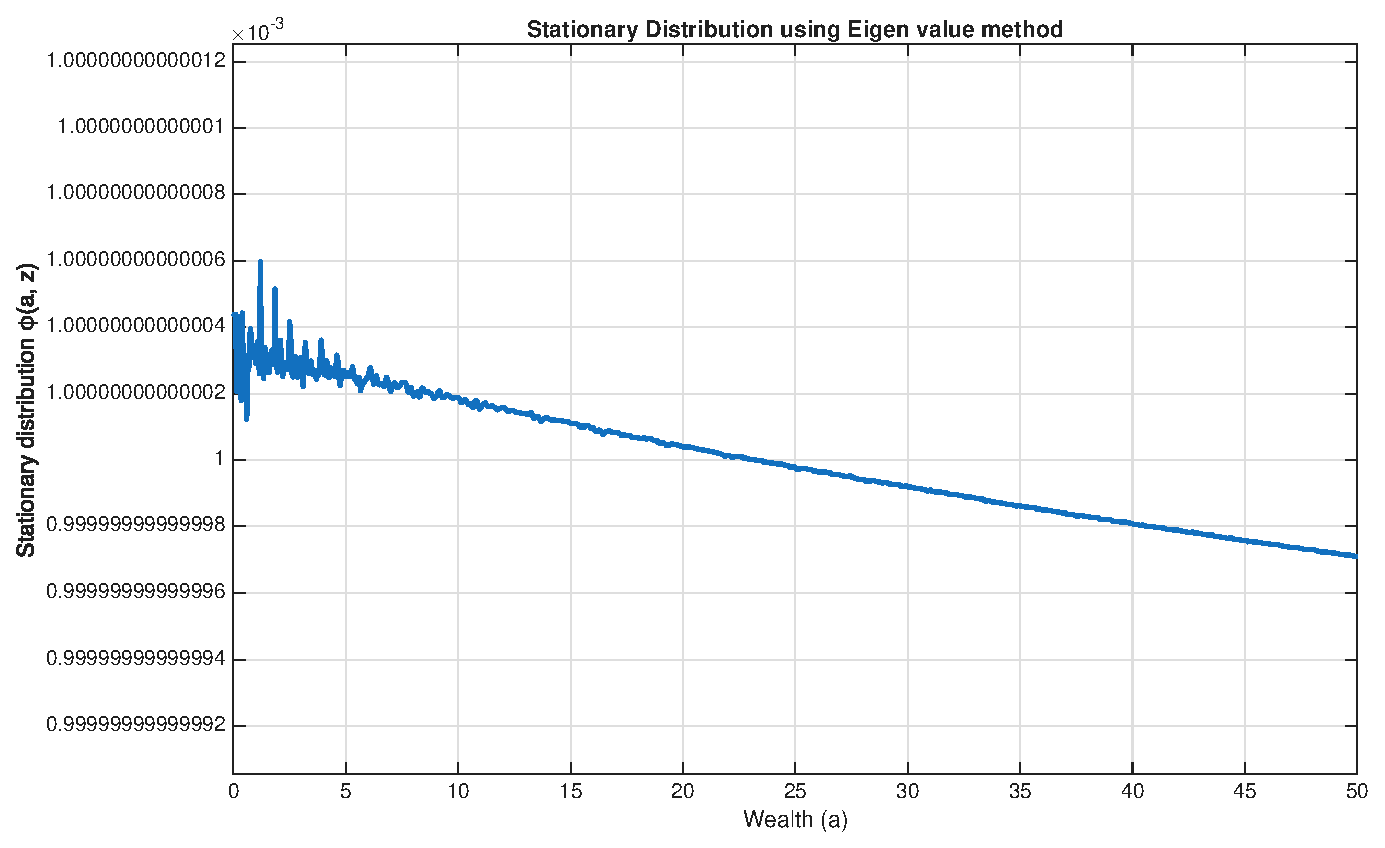
\includegraphics [width=4in]{PS3_run_01.eps}



\end{document}

